% !TeX root = ../regression_logistique.tex
\chapter{Classification multiclasse et évaluation}
\label{ch:predire}

\orient{%
appliquer la même descente aux quatre classes et combiner les résultats par
argmax ; construire un découpage stratifié ; ajuster les statistiques de
préparation sur l'apprentissage seul ; lire une matrice de confusion et
l'assortir d'une incertitude ; arbitrer un seuil de décision binaire}{%
chapitres~\ref{ch:classifieur} et~\ref{ch:entrainer}}{%
cahier pratique ; le protocole d'évaluation se met en place ici}

La boucle précédente traite une question binaire. La classification multiclasse
en ajuste quatre, les combine en une réponse unique, puis mesure cette réponse
sur des lignes absentes de l'ajustement.

\section{Extension un-contre-tous}

La descente, le coût et le gradient sont ceux de l'étape précédente, appelés
quatre fois de suite. Seule la colonne des réponses est refaite à chaque tour :
elle vaut $1$ pour la maison traitée et $0$ pour les trois autres.

\begin{tache}{Quatre descentes et l'argmax}
\tlab{Contrat} \texttt{train(X, houses)} rend un jeu de coefficients par classe,
dans l'ordre de \texttt{HOUSES}. \texttt{predict(models, x)} rend le libellé de
la classe dont le score est le plus élevé.

\tlab{Contrôle}
\begin{center}\ttfamily\footnotesize
\begin{tabular}{@{}llll@{}}
Gryffindor & cost 0.1073 & 983 iterations\\
Hufflepuff & cost 0.1368 & 779 iterations\\
Ravenclaw & cost 0.1309 & 818 iterations\\
Slytherin & cost 0.1353 & 814 iterations\\
\end{tabular}\\[3pt]
1540 students out of 1600, that is 0.9625
\end{center}
Les quatre pertes sont du même ordre ; chaque descente atteint le critère de
stagnation avant le plafond d'itérations.

\tlab{Indice 1} Le tableau \texttt{X} est construit une seule fois : seule la
colonne \texttt{target} change d'une classe à l'autre.

\tlab{Indice 2} \texttt{predict} compare directement les scores. La croissance
de $\sigma$, commune aux quatre modèles, conserve leur classement.

\tlab{Transfert} Une cinquième classe est ajoutée au fichier. Combien de
descentes, combien de coefficients, et quelles lignes de \texttt{train} et de
\texttt{predict} changent ?
\corrige{step8\_four\_houses.py}
\end{tache}

Ce taux de $0{,}9625$ est l'exactitude sur l'échantillon d'ajustement : il porte
sur les lignes qui ont servi à placer les quatre frontières. L'étape suivante le
mesure hors échantillon.

\begin{figure}[htbp]
\centering
\begin{graphique}{Quatre lignes colorées portant chacune trois coefficients, une par maison, suivies du score obtenu par l'élève 3 : +1,431, -10,181, -8,872 et -0,573. Une flèche mène du groupe des scores à un bloc predict affichant Gryffindor.}
\begin{tikzpicture}[
  house/.style={font=\footnotesize\bfseries,anchor=east,text width=24mm,
    align=right},
  row/.style={rounded corners=2pt,inner sep=4.5pt,font=\footnotesize,
    text width=48mm,align=center},
  sc/.style={font=\small,anchor=west,text width=21mm},
  res/.style={draw=gryff!55,fill=gryff!10,rounded corners=2.5pt,align=center,
    font=\small,inner sep=6pt,text width=26mm},
  arr/.style={-{Latex[length=2mm]},thick,ink!55}]

\node[row,fill=gryff!10,draw=gryff!40] (r1)
  {$-5{,}176\quad-3{,}746\quad+3{,}787$};
\node[row,fill=huffle!10,draw=huffle!40,below=2mm of r1] (r2)
  {$-3{,}103\quad+3{,}946\quad-4{,}422$};
\node[row,fill=raven!10,draw=raven!40,below=2mm of r2] (r3)
  {$-3{,}800\quad+4{,}143\quad+3{,}931$};
\node[row,fill=slyth!10,draw=slyth!40,below=2mm of r3] (r4)
  {$-4{,}627\quad-3{,}399\quad-3{,}621$};

\node[house,left=2mm of r1] {\Gryf};
\node[house,left=2mm of r2] {\Huff};
\node[house,left=2mm of r3] {\Rav};
\node[house,left=2mm of r4] {\Slyth};

\node[sc,right=3mm of r1] (s1) {$\mathbf{+1{,}431}$};
\node[sc,right=3mm of r2] (s2) {$-10{,}181$};
\node[sc,right=3mm of r3] (s3) {$-8{,}872$};
\node[sc,right=3mm of r4] (s4) {$-0{,}573$};

\coordinate (mm) at ($(s1.east)!0.5!(s4.east)$);
\node[res,right=8mm of mm] (out) {\texttt{predict}\\[1pt] \Gryf};
\draw[arr] (mm) -- (out);
\node[font=\footnotesize,text=ink,above=1.5mm of r1] {quatre jeux de coefficients};
\node[font=\footnotesize,text=ink,above=1.5mm of s1] {scores};
\end{tikzpicture}
\end{graphique}
\caption{L'élève $3$ passé aux quatre modèles, état \Movr. \Slyth arrive
deuxième : ses coefficients partagent le signe de \Gryf sur \Herb et s'y
opposent sur \Runes.}
\label{fig:ovr}
\end{figure}
\FloatBarrier

\texttt{predict} retient le plus grand des quatre scores. Comparer les scores ou
les probabilités donne le même classement, la sigmoïde étant croissante et
commune aux quatre modèles. La comparabilité des probabilités \emph{entre}
modèles relève d'une condition distincte (ch.~\ref{ch:classifieur}) ; leur calcul
est réservé à l'affichage.

\section{Mesure sur des lignes mises de côté}

La mesure hors échantillon scinde le fichier en un \emph{ensemble
d'apprentissage}, qui sert à tout ajuster, et un \emph{ensemble de test} mis de
côté avant toute opération et consulté une seule fois.

\begin{figure}[htbp]
\centering
\begin{graphique}{Schéma descendant. Le fichier brut de 1600 lignes se sépare en apprentissage, 1280 lignes, et test, 320 lignes. Du côté apprentissage, les statistiques puis les coefficients sont ajustés. Deux flèches en pointillé transportent ces nombres figés vers le côté test, qui aboutit à une exactitude lue une seule fois.}
\begin{tikzpicture}[font=\footnotesize,
  st/.style={draw=ink!30,rounded corners=2pt,align=center,font=\scriptsize,
    inner sep=4pt,text width=30mm,minimum height=8mm},
  arr/.style={-{Latex[length=1.8mm]},ink!60}]
\node[st,fill=gridgray!18] (f) {fichier brut\\ $1\,600$ lignes};
\node[st,fill=accentlight,below left=8mm and 4mm of f] (a)
  {apprentissage\\ $1\,280$ lignes};
\node[st,fill=warninglight,below right=8mm and 4mm of f] (t)
  {test\\ $320$ lignes};
\draw[arr] (f) -- (a); \draw[arr] (f) -- (t);
\node[st,fill=accentlight,below=7mm of a] (s)
  {médiane, moyenne, écart-type\\ \emph{ajustés ici}};
\node[st,fill=accentlight,below=7mm of s] (m) {coefficients ajustés};
\draw[arr] (a) -- (s); \draw[arr] (s) -- (m);
\node[st,fill=warninglight,below=25.5mm of t] (u)
  {transformation appliquée\\ avec ces mêmes nombres};
\draw[arr,densely dashed] (s.east) -- ++(6mm,0) |- (u.west);
\node[st,fill=gryff!14,below=7mm of u] (e) {exactitude\\ lue une seule fois};
\draw[arr] (u) -- (e);
\draw[arr,densely dashed] (m.east) -- ++(4mm,0) |- (e.west);
\end{tikzpicture}
\end{graphique}
\caption{Les statistiques de préparation sont des paramètres ajustés au même
titre que les coefficients. Les flèches en pointillé transportent des nombres
figés, jamais un nouvel ajustement.}
\label{fig:protocole}
\end{figure}
\FloatBarrier

Le découpage porte sur les \emph{indices}, avant toute lecture des notes. Les
statistiques de préparation sont ensuite ajustées sur les seuls indices
d'apprentissage, puis appliquées aux deux ensembles.

\begin{figure}[htbp]
\centering
\begin{graphique}{Quatre barres horizontales, une par maison, chacune partagée en une portion pleine d'apprentissage et une portion claire de test : 262 et 65 pour Gryffindor, 423 et 106 pour Hufflepuff, 354 et 89 pour Ravenclaw, 241 et 60 pour Slytherin.}
\begin{tikzpicture}[y=9mm,font=\footnotesize]
\foreach \i/\house/\col/\a/\b/\na/\nb in {%
  0/Gryffindor/gryff/4.95/6.18/262/65,
  1/Hufflepuff/huffle/8.00/10.00/423/106,
  2/Ravenclaw/raven/6.69/8.37/354/89,
  3/Slytherin/slyth/4.55/5.69/241/60}{
  \fill[\col!70] (0,-\i) rectangle (\a,-\i+0.6);
  \fill[\col!22] (\a,-\i) rectangle (\b,-\i+0.6);
  \draw[\col!45] (0,-\i) rectangle (\b,-\i+0.6);
  \node[anchor=east,text=\col,font=\footnotesize\bfseries]
    at (-1.5mm,-\i+0.3) {\house};
  \node[anchor=center,text=white,font=\scriptsize\bfseries]
    at (\a/2,-\i+0.3) {\na};
  \node[anchor=west,text=ink,font=\scriptsize,xshift=1.5mm]
    at (\b,-\i+0.3) {\nb};
}
\end{tikzpicture}
\end{graphique}
\caption{Teinte pleine, les $1\,280$ élèves d'apprentissage ; teinte claire, les
$320$ mis de côté. Le tirage stratifié prend $80\,\%$ de chaque maison, ce qui
fixe les quatre proportions d'une exécution à l'autre.}
\label{fig:decoupe}
\end{figure}
\FloatBarrier

Le mélange se fait sur les indices, par un générateur écrit sur place plutôt
que par \texttt{random.}\allowbreak\texttt{shuffle}. Chaque nombre tiré s'obtient du précédent par
\[
  \text{\'etat}\;\longleftarrow\;(a\,\text{\'etat}+c)\bmod 2^{31},
\]
avec deux constantes éprouvées. Repartir du même état initial --- la graine $0$
--- redonne la même suite, donc le même découpage à chaque exécution, condition
de comparabilité entre deux mesures.

\begin{tache}{Découpage stratifié et exactitude hors échantillon}
\tlab{Contrat} \texttt{split(houses, seed)} rend deux listes d'indices,
apprentissage et test, contenant $80\,\%$ et $20\,\%$ de \emph{chaque} classe.
Le programme ajuste ensuite \texttt{fit\_stats} sur les seuls indices
d'apprentissage, appelle \texttt{design} sur les deux ensembles, entraîne, et
mesure trois exactitudes.

\tlab{Contrôle}
\begin{center}\ttfamily\footnotesize
1280 students to learn from, 320 set aside\\
median, mean and sd fitted on the learning rows only\\[3pt]
on students already seen : 0.9609\\
on students never seen\ \ \ : 0.9719\\
everyone into Hufflepuff : 0.3312
\end{center}

\tlab{Indice 1} Grouper les indices par classe, mélanger chaque groupe, puis
prendre les quatre premiers cinquièmes de chacun : le découpage porte sur les
indices, avant toute lecture des notes.

\tlab{Indice 2} Un seul appel à \texttt{fit\_stats}, deux appels à
\texttt{design}. Un second appel à \texttt{fit\_stats} sur le test annulerait
tout le protocole.

\tlab{Transfert} Le tirage stratifié est remplacé par un tirage global de
$20\,\%$. Quelle classe voit sa part varier le plus d'une graine à l'autre, et
pourquoi ? Estimer l'effet sur la largeur de l'intervalle de Wilson.
\corrige{step9\_holdout.py}
\end{tache}

\begin{figure}[htbp]
\centering
\begin{graphique}{Un axe horizontal gradué de 0,30 à 1,00 portant trois points : le plancher à 0,3312, puis très près l'un de l'autre l'apprentissage à 0,9609 et le test à 0,9719.}
\begin{tikzpicture}[x=14.5cm,font=\footnotesize]
\draw[ink!40] (0,0) -- (1,0);
\foreach \v/\lab in {0/{0{,}30},0.2857/{0{,}50},0.6429/{0{,}75},1/{1{,}00}}{
  \draw[ink!40] (\v,-1.2mm) -- (\v,1.2mm);
  \node[anchor=north,font=\scriptsize,text=ink] at (\v,-1.8mm) {\lab};
}
\fill[ink!55] (0.0446,0) circle (1.4pt);
\node[anchor=south,align=center,text=ink,font=\scriptsize] at (0.0446,2.5mm)
  {plancher\\ $0{,}3312$};
\fill[warning] (0.9441,0) circle (1.4pt);
\fill[accent] (0.9599,0) circle (1.4pt);
\draw[warning!70] (0.9441,0) -- ++(0,7mm) -- ++(-14mm,0)
  node[anchor=east,text=warning,font=\scriptsize] {apprentissage $0{,}9609$};
\draw[accent!70] (0.9599,0) -- ++(0,-7mm) -- ++(-14mm,0)
  node[anchor=east,text=accent,font=\scriptsize] {test $0{,}9719$};
\end{tikzpicture}
\end{graphique}
\caption{Plancher : exactitude d'une règle attribuant \Huff à tout le monde. L'écart
apprentissage-test vaut onze millièmes, soit trois ou quatre élèves sur $320$.}
\label{fig:echelle}
\end{figure}
\FloatBarrier

Le premier chiffre est l'exactitude sur l'échantillon d'ajustement, optimiste
par construction. Le deuxième porte sur $320$ observations absentes de
l'ajustement : c'est celui qui prédit une observation à venir. Le troisième donne le
plancher, obtenu par une règle qui met tout le monde dans la classe majoritaire ;
un modèle doit le dépasser nettement pour démontrer un apport.

Ici le second dépasse le premier, d'un écart qui reste dans la marge d'un
échantillon de $320$ lignes. Un modèle à $99\,\%$ sur l'apprentissage et
$85\,\%$ sur le test aurait au contraire ajusté le bruit des lignes vues plutôt
que la régularité : c'est le \emph{surapprentissage}.

Cet écart en est un révélateur parmi d'autres, souvent moins sensible qu'une
courbe d'apprentissage, une validation croisée, la comparaison des pertes ou la
stabilité des coefficients d'un découpage à l'autre. Trois coefficients par
classe offrent peu de liberté, et le surapprentissage tient aussi à la sélection
des variables, au réglage répété sur les mêmes données, à un échantillon petit ou
bruité. Les deux matières employées ici ont été choisies après examen du fichier
étiqueté entier : ce canal précède le découpage, et l'écart apprentissage-test
reste par construction aveugle à son effet. Un protocole complet choisirait les
variables sur les seules lignes d'apprentissage, ou sur un ensemble de validation
distinct du test.

\section{Résultats et limites}

Un taux global agrège des erreurs de natures différentes et laisse sa propre
précision indéterminée. Deux compléments le complètent, et tiennent en une
trentaine de lignes.

\textbf{La matrice de confusion} croise classe observée et classe prédite. Ses
seize cases distinguent une classe systématiquement manquée d'erreurs réparties
au hasard, ce que le taux global confond.

\begin{table}[htbp]
\centering
\begin{tabular}{lrrrrr}
\toprule
& \multicolumn{4}{c}{\textbf{prédite}} & \\
\cmidrule(lr){2-5}
\textbf{observée} & \Gryf & \Huff & \Rav & \Slyth & total \\
\midrule
\Gryf  & $\mathbf{62}$ & $1$ & $2$ & $0$ & $65$ \\
\Huff  & $0$ & $\mathbf{105}$ & $1$ & $0$ & $106$ \\
\Rav   & $0$ & $2$ & $\mathbf{86}$ & $1$ & $89$ \\
\Slyth & $0$ & $2$ & $0$ & $\mathbf{58}$ & $60$ \\
\bottomrule
\end{tabular}
\caption{Matrice de confusion sur les $320$ lignes mises de côté ; diagonale en
gras, $311$ prédictions correctes. Les neuf erreurs se répartissent inégalement :
trois \Gryf manqués, cinq prédictions \Huff excédentaires.}
\label{tab:confusion}
\end{table}

\textbf{L'incertitude.} Pour $311$ succès sur $320$ lignes, l'intervalle de
Wilson à $95\,\%$~\cite{wilson1927} vaut
\[
  [0{,}9474\,;0{,}9851].
\]
Sa largeur, proche de quatre points, donne la précision justifiée par
l'effectif.

\begin{table}[htbp]
\centering
\begin{tabular}{lrrrr}
\toprule
classe & rappel & précision & $F_1$ & effectif \\
\midrule
\Gryf  & $0{,}9538$ & $1{,}0000$ & $0{,}9764$ & $65$ \\
\Huff  & $0{,}9906$ & $0{,}9545$ & $0{,}9722$ & $106$ \\
\Rav   & $0{,}9663$ & $0{,}9663$ & $0{,}9663$ & $89$ \\
\Slyth & $0{,}9667$ & $0{,}9831$ & $0{,}9748$ & $60$ \\
\bottomrule
\end{tabular}
\caption{Mesures par classe. Le \emph{rappel} est la part d'une classe
retrouvée, la \emph{précision} la part des prédictions d'une classe qui lui
reviennent. Sur ces effectifs, les écarts restent dans la marge
d'échantillonnage.}
\label{tab:parclasse}
\end{table}

\begin{tache}{Matrice de confusion et incertitude}
\tlab{Contrat} À partir des prédictions sur le test, produire la matrice
$4\times4$ observée $\times$ prédite, les couples rappel-précision par classe,
l'exactitude globale, son intervalle de Wilson à $95\,\%$ et le plancher de la
classe majoritaire.

\tlab{Contrôle}
\begin{center}\ttfamily\footnotesize
accuracy 311/320 = 0.9719\ \ \ Wilson 95\% [0.9474 ; 0.9851]\\
baseline, everyone into Hufflepuff: 0.3312
\end{center}
Les seize cases doivent totaliser $320$, et la diagonale $311$.

\tlab{Indice 1} Indexer la matrice par la position de la classe dans
\texttt{HOUSES}, non par son libellé : les totaux de ligne et de colonne
s'obtiennent alors par simple somme.

\tlab{Indice 2} L'intervalle de Wilson pour $k$ succès sur $n$ tirages s'écrit
avec $z_{0{,}975}=1{,}96$ ; il n'est pas symétrique autour de $k/n$, ce qui se
vérifie sur les bornes attendues.

\tlab{Transfert} Une classe obtient un rappel de $0{,}55$ pour une précision de
$0{,}98$. Décrire le comportement du modèle sur cette classe, dire quelle case de
la matrice le révèle, et indiquer si déplacer un seuil pourrait le corriger.
\corrige{step10\_evaluation.py}
\end{tache}

La portée de ces chiffres s'arrête à trois limites. Un seul découpage mesure un
seul découpage : plusieurs graines, ou une validation croisée à $k$ blocs,
donneraient en outre une dispersion. Le choix des deux matières reste antérieur
au découpage. Et la calibration reste à vérifier, de sorte que les probabilités
affichées valent pour leur ordre plutôt que comme des fréquences.

\section{Seuil de décision, en binaire}

Le classifieur à quatre classes tranche par comparaison de scores. Sur le
sous-problème binaire du chapitre~\ref{ch:probabilite}, la conversion d'une
probabilité en réponse demande un \emph{seuil} : au-dessus, la classe prédite
est \Gryf. Le cours adopte $s=0{,}5$, ce qui compte les deux erreurs au même
prix.

Le seuil se fixe après l'entraînement, qui détermine les coefficients et avec eux
les probabilités. Les mêmes probabilités, lues avec deux seuils, donnent deux
classements.

Sur $0{,}5$, la comparaison se ramène au signe du score,
\[
  p\geq0{,}5 \iff z\geq0 \iff \text{l'observation appartient au demi-plan \Gryf},
\]
les trois formulations étant équivalentes puisque $\sigma$ est croissante et vaut
$0{,}5$ en zéro. Le programme peut donc s'en tenir aux scores lorsque seule la
maison intéresse, et calculer les probabilités uniquement pour les afficher.

Déplacer le seuil échange une erreur contre l'autre, les deux portant sur des
observations distinctes : un \Gryf dont la probabilité tombe sous le seuil est
manqué, une observation d'une autre classe dont la probabilité le dépasse est
désignée à tort. Monter le seuil raréfie les secondes et multiplie les
premières ; le descendre produit l'effet inverse. Choisir un seuil revient donc
à choisir la proportion entre les deux.

\begin{figure}[htbp]
\centering
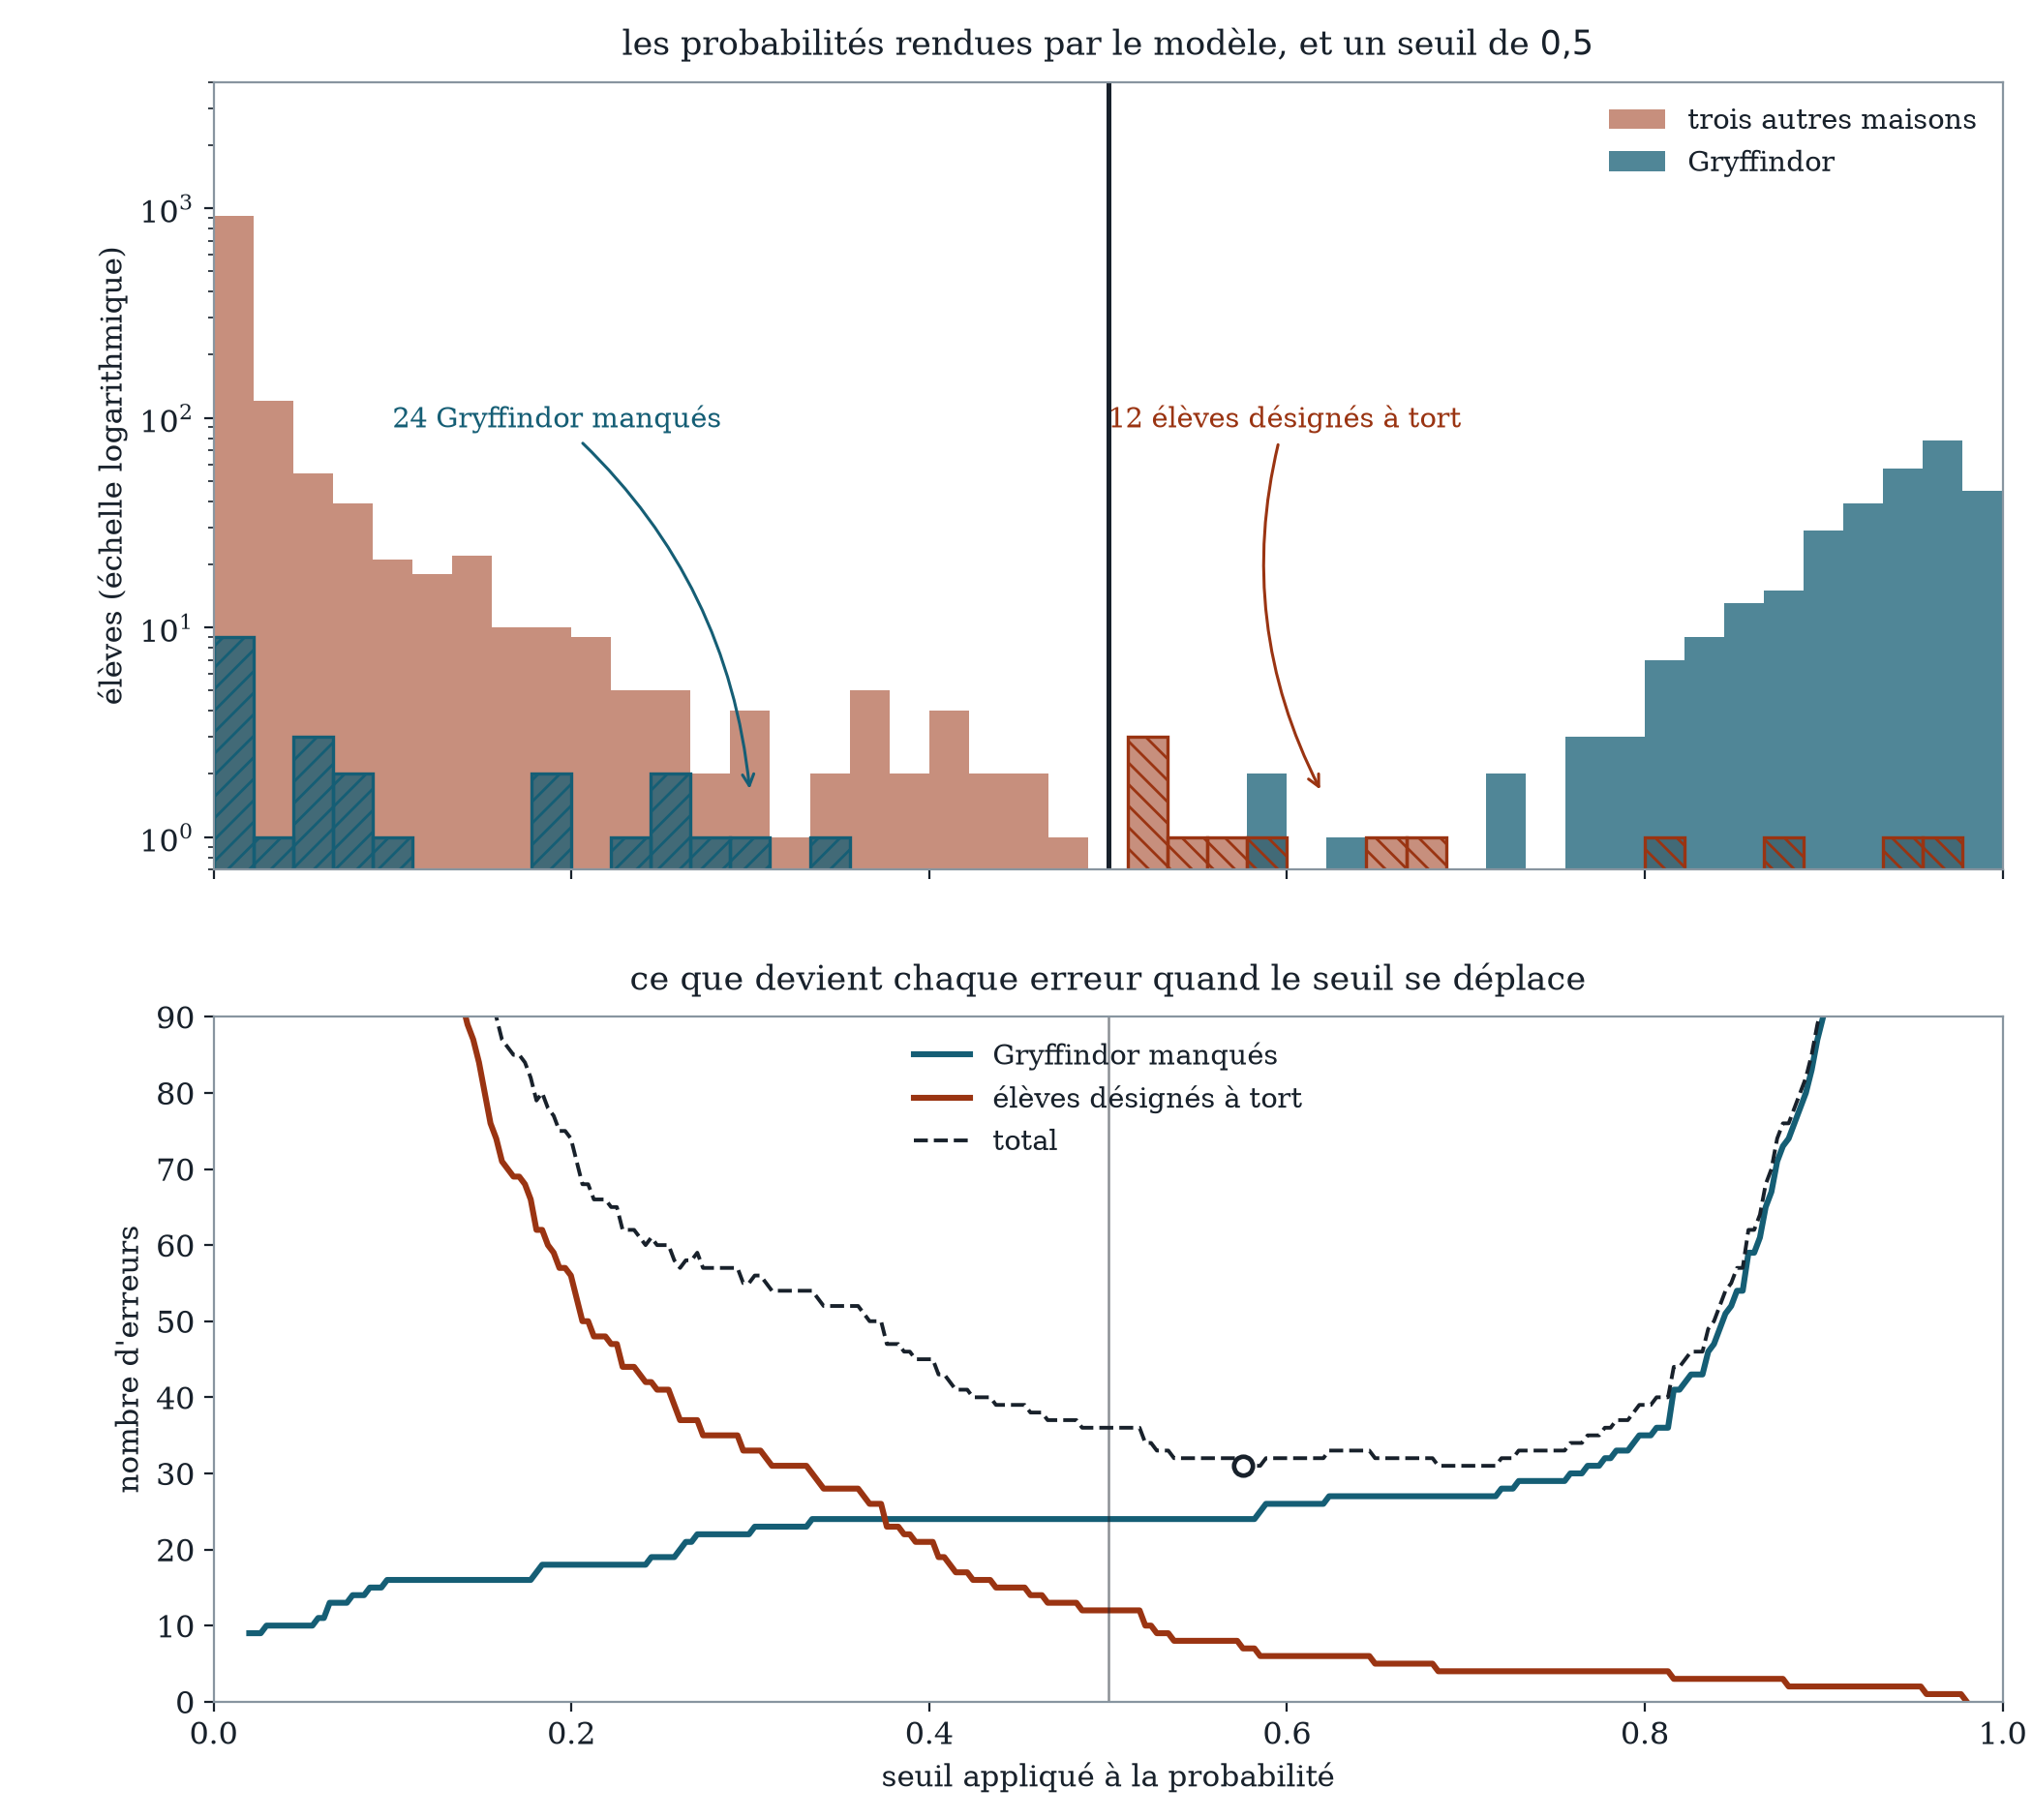
\includegraphics[width=\textwidth,
  alt={Deux panneaux à axe horizontal commun, la probabilité rendue par le modèle. En haut, deux histogrammes en échelle logarithmique séparés selon la classe observée, hachures sur les prédictions incorrectes au seuil 0,5. En bas, deux courbes d'erreurs de sens contraire selon le seuil, et leur somme dont le minimum est cerclé vers 0,58.}]{figures/seuil.png}
\caption{Probabilités par classe observée, en haut ; hachures : erreurs au seuil
$0{,}5$. Nombre d'erreurs selon le seuil, en bas ; minimum cerclé.}
\label{fig:seuil}
\end{figure}
\FloatBarrier

Un seuil $s$ quelconque revient de même à comparer le score au logit de $s$, donc
à tracer la droite $z=\operatorname{logit}(s)$, parallèle à celle de $0{,}5$.
Changer le seuil translate la frontière sans la faire pivoter, ce qui revient à
déplacer le seul biais $w_0$ (ch.~\ref{ch:nuage}).

\begin{figure}[htbp]
\centering
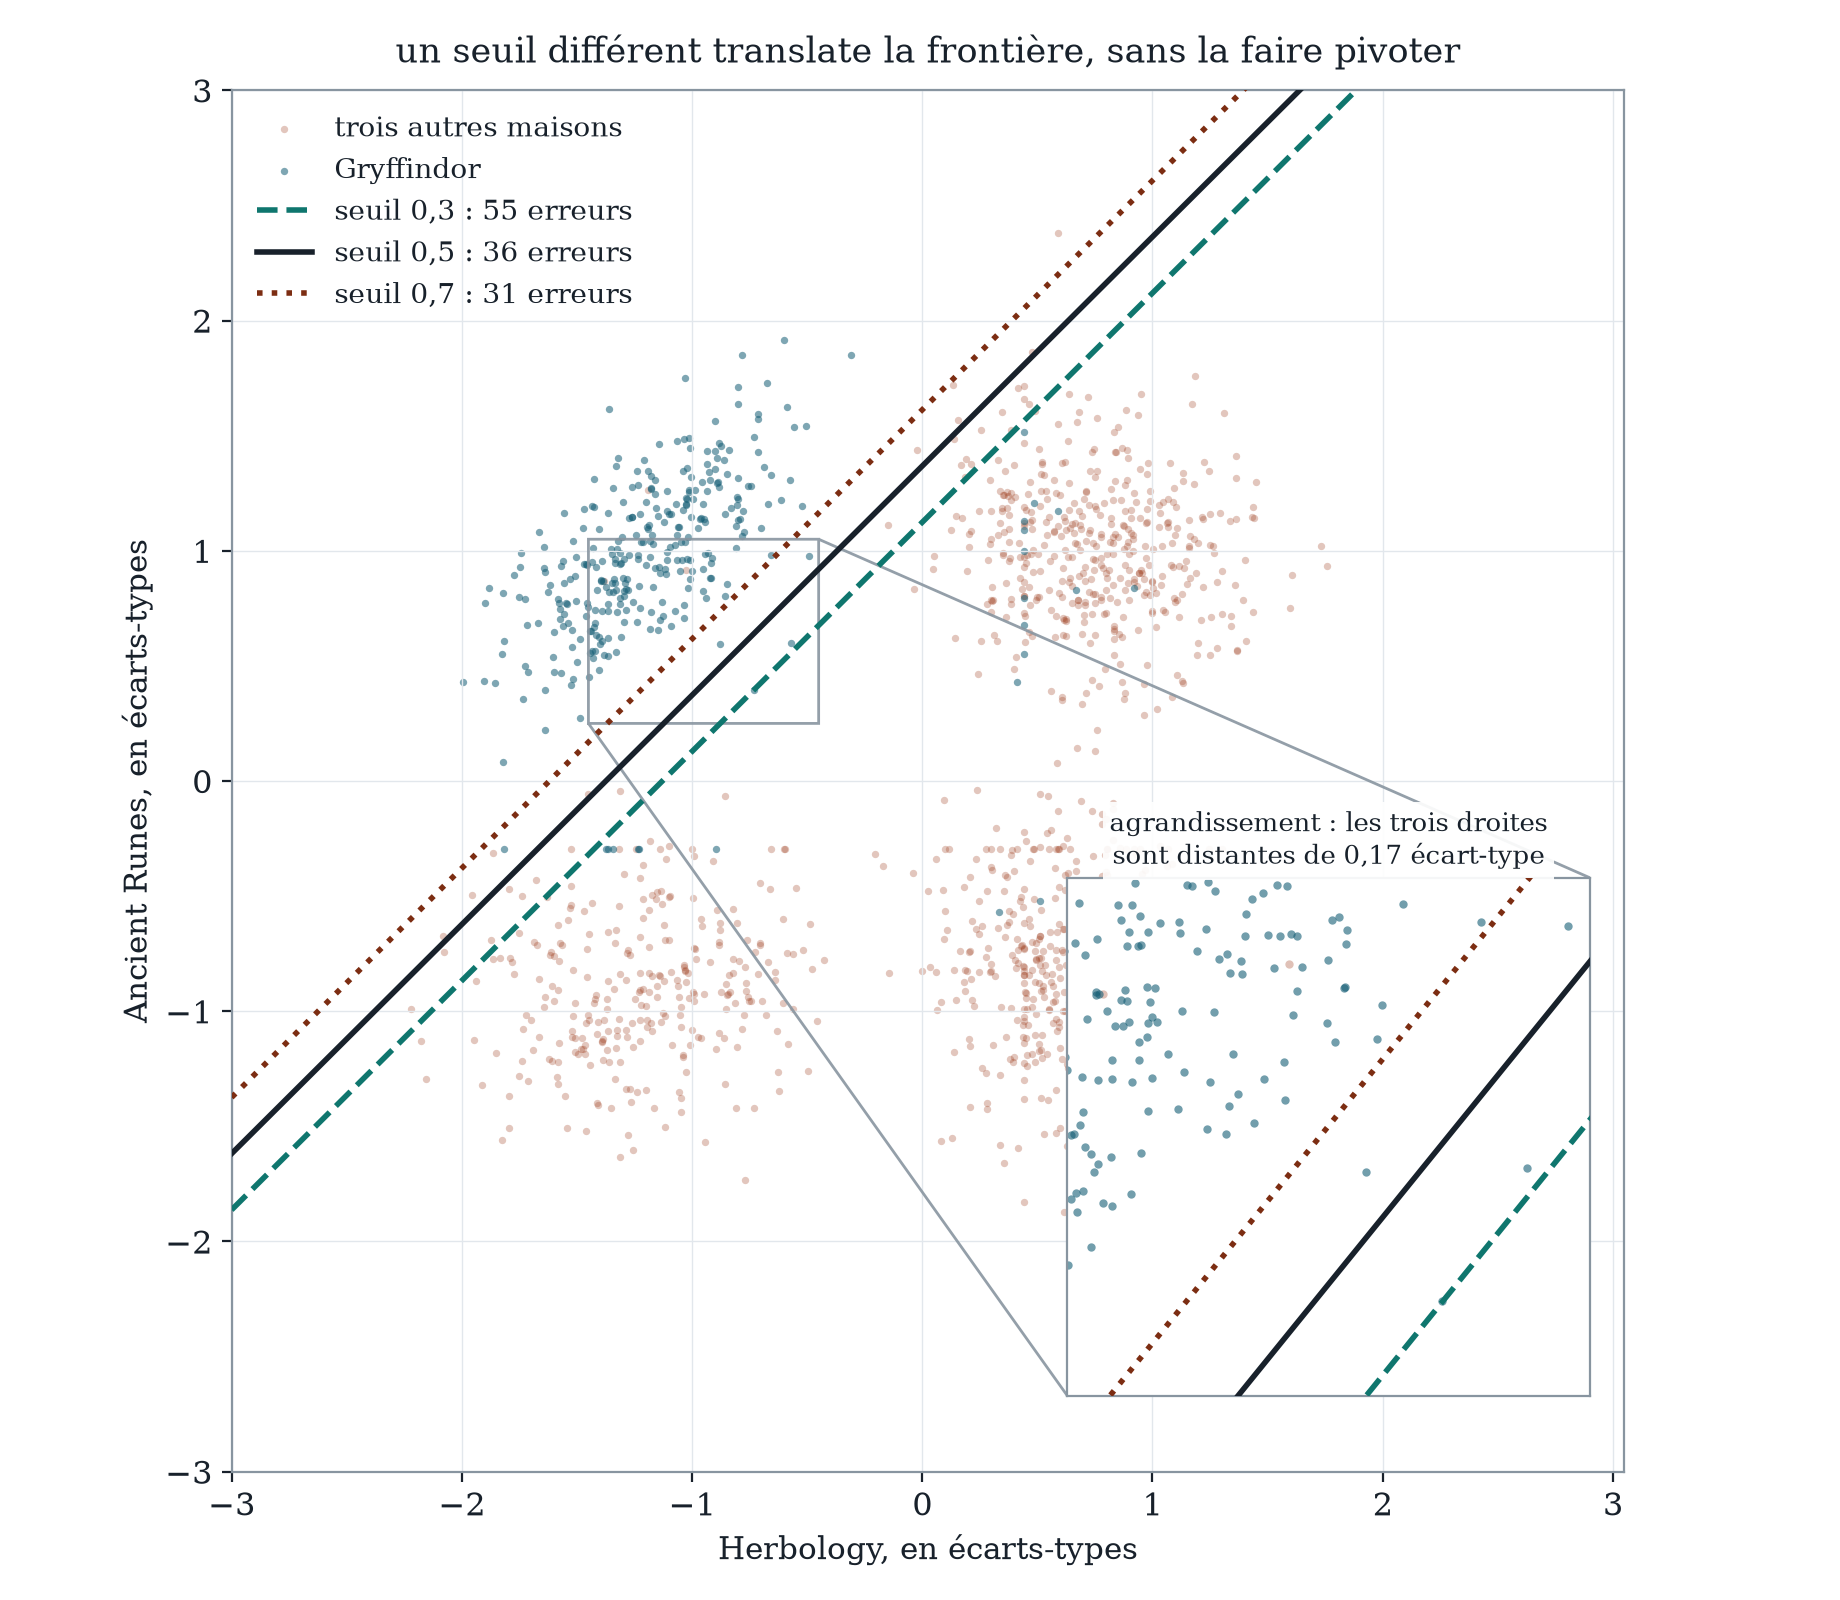
\includegraphics[width=\textwidth,
  alt={Nuage standardisé traversé par trois droites parallèles correspondant aux seuils 0,3, 0,5 et 0,7. Un agrandissement montre la poignée d'observations comprises entre elles, qui changent de réponse d'un seuil à l'autre.}]{figures/seuil_plan.png}
\caption{Nuage standardisé et droites des seuils $0{,}3$, $0{,}5$ et $0{,}7$ :
même direction, biais décalés. L'agrandissement porte les observations qui
changent de réponse d'une droite à l'autre.}
\label{fig:seuil-plan}
\end{figure}
\FloatBarrier

\begin{releve}
Les trois seuils reviennent aux biais $-3{,}898$, $-4{,}745$ et $-5{,}593$, soit
des droites distantes de $0{,}17$ écart-type.
\end{releve}

\begin{chiffres}[Erreurs selon le seuil, état \Mquatre]
\begin{center}
\begin{tabular}{crrrl}
\toprule
seuil & \Gryf manqués & désignés à tort & total & \\
\midrule
$0{,}30$ & $22$ & $33$ & $55$ & \\
$0{,}50$ & $24$ & $12$ & $36$ & seuil retenu \\
$0{,}58$ & $24$ & $7$  & $31$ & \\
$0{,}5824$ & $23$ & $7$ & $30$ & minimum sur ce fichier \\
$0{,}70$ & $27$ & $4$  & $31$ & \\
\bottomrule
\end{tabular}
\end{center}
Le minimum n'apparaît qu'en balayant les seuils au dix-millième ; une grille plus
grossière rend $31$. Un seuil obtenu par balayage sur les données d'ajustement
est une valeur ajustée de plus, qui se déplacerait sur un autre échantillon.
\end{chiffres}

L'origine de ce décalage tient à l'échantillon, non au déséquilibre des classes.
Sous des probabilités conditionnelles correctement estimées et deux erreurs
comptées au même prix, le seuil qui minimise le nombre d'erreurs vaut $0{,}5$
quel que soit le déséquilibre : c'est la règle de décision de Bayes, et les
proportions de classes n'y interviennent pas. Le rapport de $327$ \Gryf à
$1\,273$ autres élèves est d'ailleurs déjà absorbé par le biais $w_0$, qui
s'ajuste sur la fréquence de base (ch.~\ref{ch:descente}).

Le décalage observé a trois causes : calibration imparfaite des probabilités
estimées, spécification affine approchée de la vraie frontière, et taille finie
de l'échantillon --- déplacer le seuil de $0{,}5$ à $0{,}58$ fait basculer une
poignée d'observations, l'ordre de grandeur du bruit d'échantillonnage. Le
programme garde $0{,}5$, issu d'une décision explicite plutôt que d'un ajustement
sur ce fichier.

Un seuil franchement différent se justifie lorsque les deux erreurs coûtent des
prix différents. Recenser toutes les observations d'une classe quitte à en
désigner quelques-unes de trop conduit à abaisser le seuil ; ne désigner que des
cas sûrs conduit à l'élever. Ce choix relève de l'usage fait des prédictions, que
les données seules laissent ouvert.

À quatre classes, la décision compare les quatre scores et retient le plus grand
(ch.~\ref{ch:classifieur}) ; le seuil ne s'applique donc qu'au sous-problème
binaire. La valeur $0{,}5$ garde partout son autre rôle : probabilité rendue par
$\sigma$ en zéro, elle situe la frontière et donne le coût de départ.

\section{Compléments pour un programme livrable}

Trois ajouts séparent ce qui précède d'un programme utilisable sur un fichier
d'élèves inconnus.

\textbf{Enregistrer le modèle.} Les quatre vecteurs, mais aussi les trois
statistiques par matière, la liste ordonnée des matières et celle des maisons. Un
coefficient s'applique à la note qui occupait sa place pendant l'entraînement, et
le plus grand score ne devient une maison que par la liste des libellés. Perdre
l'un de ces ordres donne des scores justes et des réponses fausses, sans aucune
erreur d'exécution.

\textbf{Appliquer les statistiques d'entraînement à la prédiction.} Un élève
inconnu reçoit la médiane, la moyenne et l'écart-type appris sur les élèves
d'entraînement, jamais les siens. Recalculer ces trois nombres sur les nouvelles
données placerait les scores dans une autre échelle ; sur un fichier d'un seul
élève, l'écart-type serait nul et l'opération n'aurait pas de sens.

\textbf{Consigner le protocole.} La graine du découpage, la proportion retenue,
les statistiques ajustées et la date de la mesure. Ces quatre éléments rendent le
chiffre annoncé reproductible, condition pour qu'il constitue un résultat.

\section{Micro-cas de transfert}
\label{sec:transfert}

Le fil rouge a fourni un seul jeu de données. Le micro-cas suivant reprend la
chaîne entière sur douze observations d'un autre domaine, dans d'autres unités,
et fait apparaître un comportement que les $1\,600$ élèves masquaient.

\begin{table}[htbp]
\centering
\small
\setlength{\tabcolsep}{5pt}
\begin{tabular}{rrc rrc rrc}
\toprule
\multicolumn{2}{c}{mesures} & classe &
\multicolumn{2}{c}{mesures} & classe &
\multicolumn{2}{c}{mesures} & classe \\
$d$ & $H$ & & $d$ & $H$ & & $d$ & $H$ & \\
\midrule
$10{,}02$ & $121$ & $0$ & $9{,}96$  & $127$ & $0$ & $10{,}35$ & $147$ & $1$ \\
$10{,}05$ & $118$ & $0$ & $10{,}07$ & $116$ & $0$ & $9{,}71$  & $145$ & $1$ \\
$9{,}98$  & $124$ & $0$ & $10{,}31$ & $143$ & $1$ & $10{,}24$ & $136$ & $1$ \\
$10{,}01$ & $119$ & $0$ & $10{,}28$ & $139$ & $1$ & $9{,}68$  & $141$ & $1$ \\
\bottomrule
\end{tabular}
\caption{Douze pièces usinées : diamètre $d$ en millimètres, dureté $H$ en
vickers, classe $1$ pour un rebut. Les deux colonnes diffèrent d'un facteur
cinquante en échelle.}
\label{tab:micro}
\end{table}

\begin{tache}{Transfert : douze pièces, deux mesures}
\tlab{Contrat} Reprendre \texttt{score\_of}, \texttt{sigmoid},
\texttt{student\_cost}, \texttt{gradient} et la boucle sans les modifier ;
n'écrire que la lecture du tableau et la standardisation des deux colonnes.

\tlab{Contrôle}
\begin{center}\ttfamily\footnotesize
diametre mean 10.0550 sd 0.2071\\
durete\ \ \ mean 131.3333 sd 11.1305\\
cost with zero weights: 0.693147\\[3pt]
stopped after 6000 iterations (plafond), cost 0.000595\\
weights: -0.2721 +1.8591 +11.6553\\
12/12 pieces classees correctement
\end{center}

\tlab{Indice 1} Le coût de départ vaut $\log 2$ ici comme ailleurs : il ne
dépend ni du nombre d'observations, ni de leurs unités.

\tlab{Indice 2} La boucle sort par le plafond, non par la stagnation. Comparer
$\|w\|$ au tour $1\,000$ et au tour $6\,000$ avant de conclure à une erreur de
programmation.

\tlab{Transfert} Les douze pièces sont linéairement séparables. Expliquer
pourquoi la perte tend vers zéro sans que la descente s'arrête, en quoi le
plafond d'itérations est ici le seul critère qui puisse trancher, et ce que
deviendrait la frontière avec un plafond dix fois plus grand
(\annexeref{ann:norme}). Prédire ensuite la classe d'une pièce mesurant
$10{,}20$~mm pour $133$~HV, puis vérifier : $x=(+0{,}700\,;+0{,}150)$ et
$z=+2{,}775$.
\corrige{transfert\_micro.py}
\end{tache}
